
%(BEGIN_QUESTION)
% Copyright 2009, Tony R. Kuphaldt, released under the Creative Commons Attribution License (v 1.0)
% This means you may do almost anything with this work of mine, so long as you give me proper credit

Beregn og tegn inn to ulike {\it lastlinjer} oppå transistorens karakteristikk-kurver: én lastlinje med 2 k$\Omega$ kollektor- (last-)motstand, og én uten kollektor-motstand i det hele tatt (dvs. konstant 20 volt mellom kollektor og emitter til enhver tid):

$$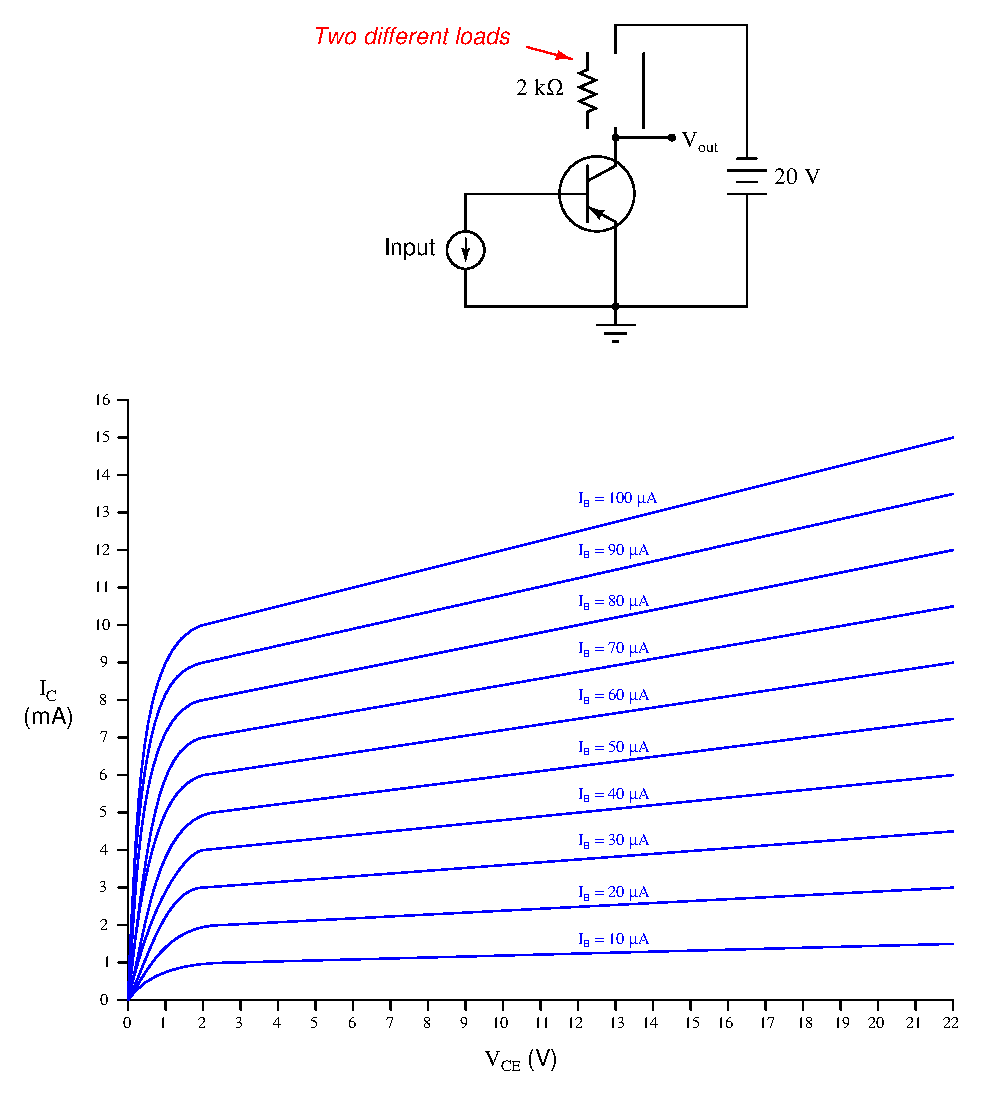
\includegraphics[width=15.5cm]{i01386x01.eps}$$

\vfil \eject

Tegn deretter to grafer som viser sammenhengen mellom basestrøm ($I_B$) og kollektorstrøm ($I_C$), én graf for hver lasttilstand (uten lastmotstand versus 2 k$\Omega$ lastmotstand). I hvilket tilfelle er sammenhengen mellom base- og kollektorstrøm mest lineær? Forklar hvorfor.

$$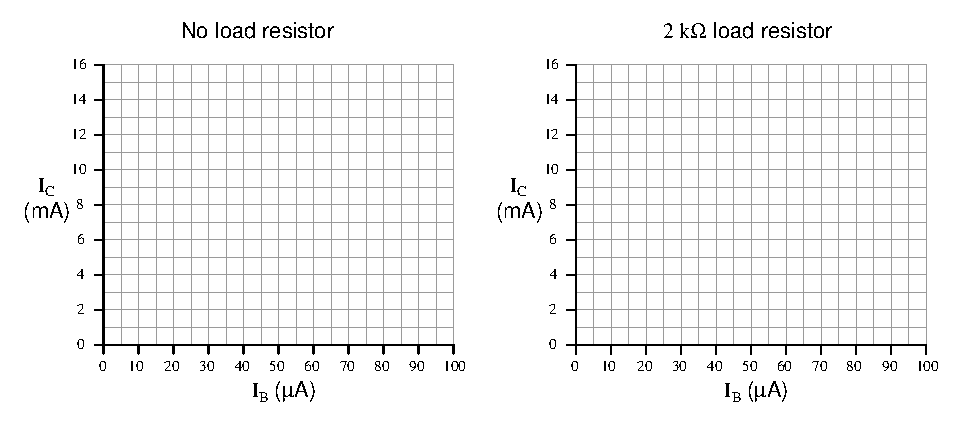
\includegraphics[width=15.5cm]{i01386x03.eps}$$

Forklar også hvordan oppførselen til denne elektroniske kretsen relaterer seg til installert versus iboende karakteristikk for reguleringsventiler. Identifiser hva hver av disse parameterne i transistorkretsen tilsvarer i et reguleringsventilscenario:

\begin{itemize}
\item{} Basestrøm
\item{} Kollektorstrøm
\item{} Kollektor-emitter-spenning
\item{} Kollektormotstand (lastverdi)
\end{itemize}

\underbar{file i01386}
%(END_QUESTION)





%(BEGIN_ANSWER)

De to lastlinjene er vist her, lagt over samme graf med karakteristikkurver:

$$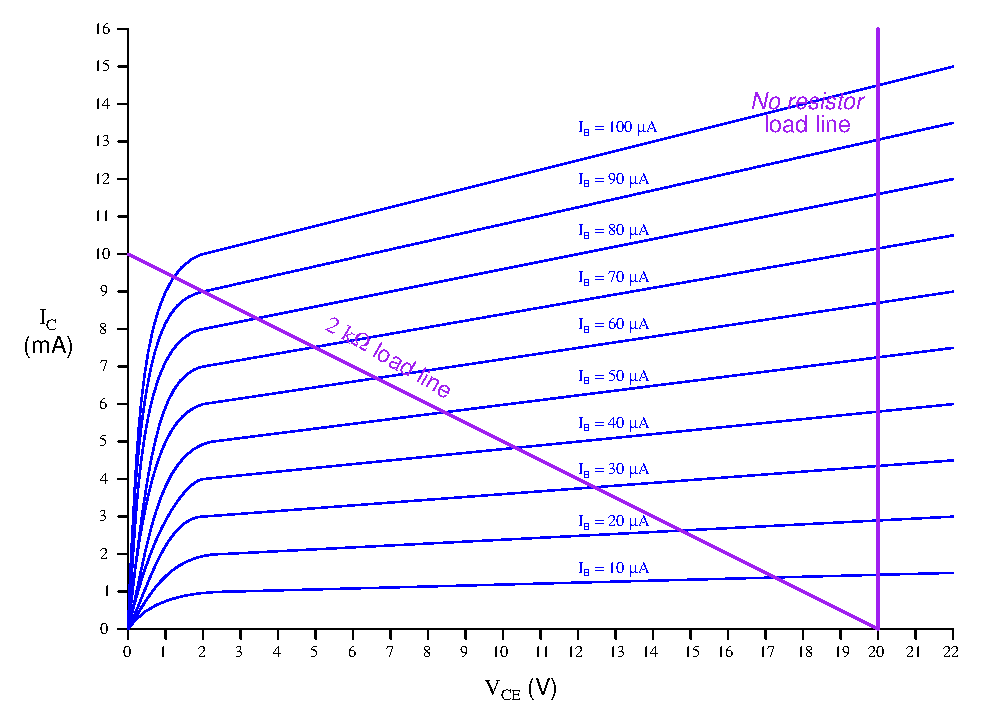
\includegraphics[width=15.5cm]{i01386x02.eps}$$

\vskip 10pt

$$\hbox{Ingen lastmotstand \hskip 70pt 2 k$\Omega$ lastmotstand}$$

% Ingen blanklinjer er tillatt mellom linjer i en \halign-struktur!
% Jeg bruker kommentarer (%) i stedet, slik at TeX ikke feiler.

$$\vbox{\offinterlineskip
\halign{\strut
\vrule \quad\hfil # \ \hfil &
\vrule \quad\hfil # \ \hfil \vrule \cr
\noalign{\hrule}
%
% Første rad
$I_B$ & $I_C$ \cr
%
\noalign{\hrule}
%
% Neste rad
10 $\mu$A & 1.4 mA \cr
%
\noalign{\hrule}
%
% Neste rad
20 $\mu$A & 2.9 mA \cr
%
\noalign{\hrule}
%
% Neste rad
30 $\mu$A & 4.4 mA \cr
%
\noalign{\hrule}
%
% Neste rad
40 $\mu$A & 5.8 mA \cr
%
\noalign{\hrule}
%
% Neste rad
50 $\mu$A & 7.25 mA \cr
%
\noalign{\hrule}
%
% Neste rad
60 $\mu$A & 8.7 mA \cr
%
\noalign{\hrule}
%
% Neste rad
70 $\mu$A & 10.1 mA \cr
%
\noalign{\hrule}
%
% Neste rad
80 $\mu$A & 11.6 mA \cr
%
\noalign{\hrule}
%
% Neste rad
90 $\mu$A & 13.1 mA \cr
%
\noalign{\hrule}
%
% Neste rad
100 $\mu$A & 14.5 mA \cr
%
\noalign{\hrule}
} % Slutt på \halign
}
\hskip 40pt
\vbox{\offinterlineskip
\halign{\strut
\vrule \quad\hfil # \ \hfil &
\vrule \quad\hfil # \ \hfil \vrule \cr
\noalign{\hrule}
%
% Første rad
$I_B$ & $I_C$ \cr
%
\noalign{\hrule}
%
% Neste rad
10 $\mu$A & 1.4 mA \cr
%
\noalign{\hrule}
%
% Neste rad
20 $\mu$A & 2.6 mA \cr
%
\noalign{\hrule}
%
% Neste rad
30 $\mu$A & 3.75 mA \cr
%
\noalign{\hrule}
%
% Neste rad
40 $\mu$A & 4.8 mA \cr
%
\noalign{\hrule}
%
% Neste rad
50 $\mu$A & 5.75 mA \cr
%
\noalign{\hrule}
%
% Neste rad
60 $\mu$A & 6.7 mA \cr
%
\noalign{\hrule}
%
% Neste rad
70 $\mu$A & 7.5 mA \cr
%
\noalign{\hrule}
%
% Neste rad
80 $\mu$A & 8.25 mA \cr
%
\noalign{\hrule}
%
% Neste rad
90 $\mu$A & 9 mA \cr
%
\noalign{\hrule}
%
% Neste rad
100 $\mu$A & 9.4 mA \cr
%
\noalign{\hrule}
} % Slutt på \halign
}
$$ % Slutt på \vbox

\vskip 10pt

\filbreak

De analoge størrelsene mellom transistorkretsen og reguleringsventilinstallasjonen er:

\begin{itemize}
\item{} Basestrøm = {\it $C_v$-verdi, som er direkte proporsjonal med spindelstilling for lineær ventiltrim}
\item{} Kollektorstrøm = {\it strømning ($Q$) gjennom ventilen}
\item{} Kollektor-emitter-spenning = {\it trykkfall ($P_1 - P_2$) over ventilen}
\item{} Kollektormotstand (lastverdi) = {\it trykktap på grunn av strømning gjennom rør, varmevekslere, pumper osv.}
\end{itemize}

$$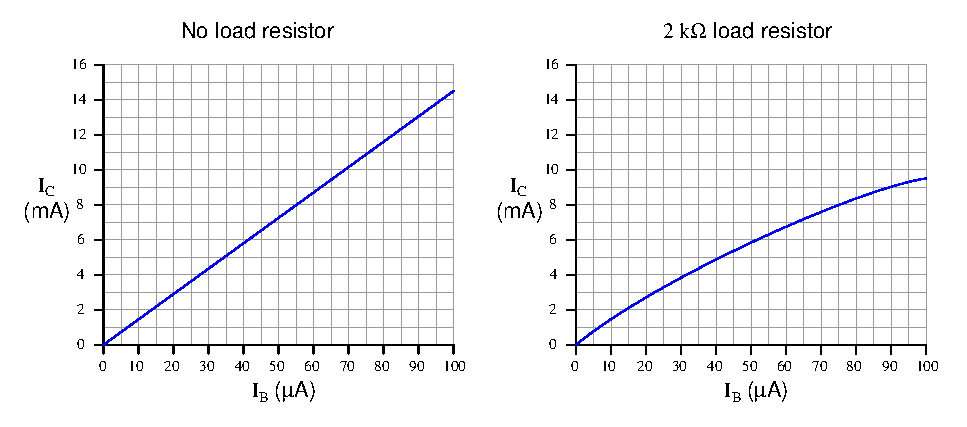
\includegraphics[width=15.5cm]{i01386x04.eps}$$

Når vi legger en lineær funksjon oppå et sett med ikke-lineære funksjoner og ser etter skjæringspunktene, kan vi løse for flere variabler i et ikke-lineært matematisk system. Vanligvis regnes bare {\it lineære} ligningssystemer som ``løselige'' uten å ty til svært tidkrevende regning, men her har vi et kraftig (grafisk) verktøy for å tilnærme variabelverdier i et ikke-lineært system. Siden tilnærminger uansett er det beste vi kan håpe på i transistorkretser, er dette godt nok!


%(END_ANSWER)





%(BEGIN_NOTES)


%INDEX% Electronics review: load lines
%INDEX% Final Control Elements, valve: characterization

%(END_NOTES)

